%mainfile: ../../master.tex
\subsection{Events}

\begin{table}[h!]
  \centering
  \begin{adjustbox}{max width=\textwidth}
    \begin{tabular}{*{15}{|l}|}
        \hline
        \textbf{Event} & Person & Action & Pattern & Mistake & Sensor & Switch & Lamp & Light intensity & Room & Premise & Time \\
        \hline
        Entered home & \cmark & \cmark & \cmark & & \cmark & & \cmark & \cmark & \cmark & \cmark & \\
        \hline
        Left home & \cmark & \cmark & \cmark & & \cmark & & \cmark & & \cmark & \cmark & \\
        \hline
        Enter room & \cmark & \cmark & \cmark & & \cmark & & \cmark & \cmark & \cmark & & \\
        \hline
        Left room & \cmark & \cmark & \cmark & & \cmark & & \cmark & \cmark & \cmark & &\\
        \hline
        Flicked switch & \cmark & \cmark & \cmark & \cmark & \cmark & \cmark & \cmark & \cmark & \cmark & & \\
        \hline
        Outside/External light intensity down & \cmark & & & & \cmark & \cmark & \cmark & \cmark & \cmark & &\\
        \hline
        Outside/External light intensity up & \cmark & & & & \cmark & \cmark & \cmark & \cmark& \cmark & &\\
        \hline
        Person sleeping & \cmark & \cmark & \cmark & & \cmark & & \cmark & & \cmark & & \cmark\\
        \hline
    \end{tabular}
  \end{adjustbox}
  \caption{Event table}
  \label{tab:eventtable}
\end{table}

\begin{figure}
   \centering
   \begin{adjustbox}{max width=\textwidth}
    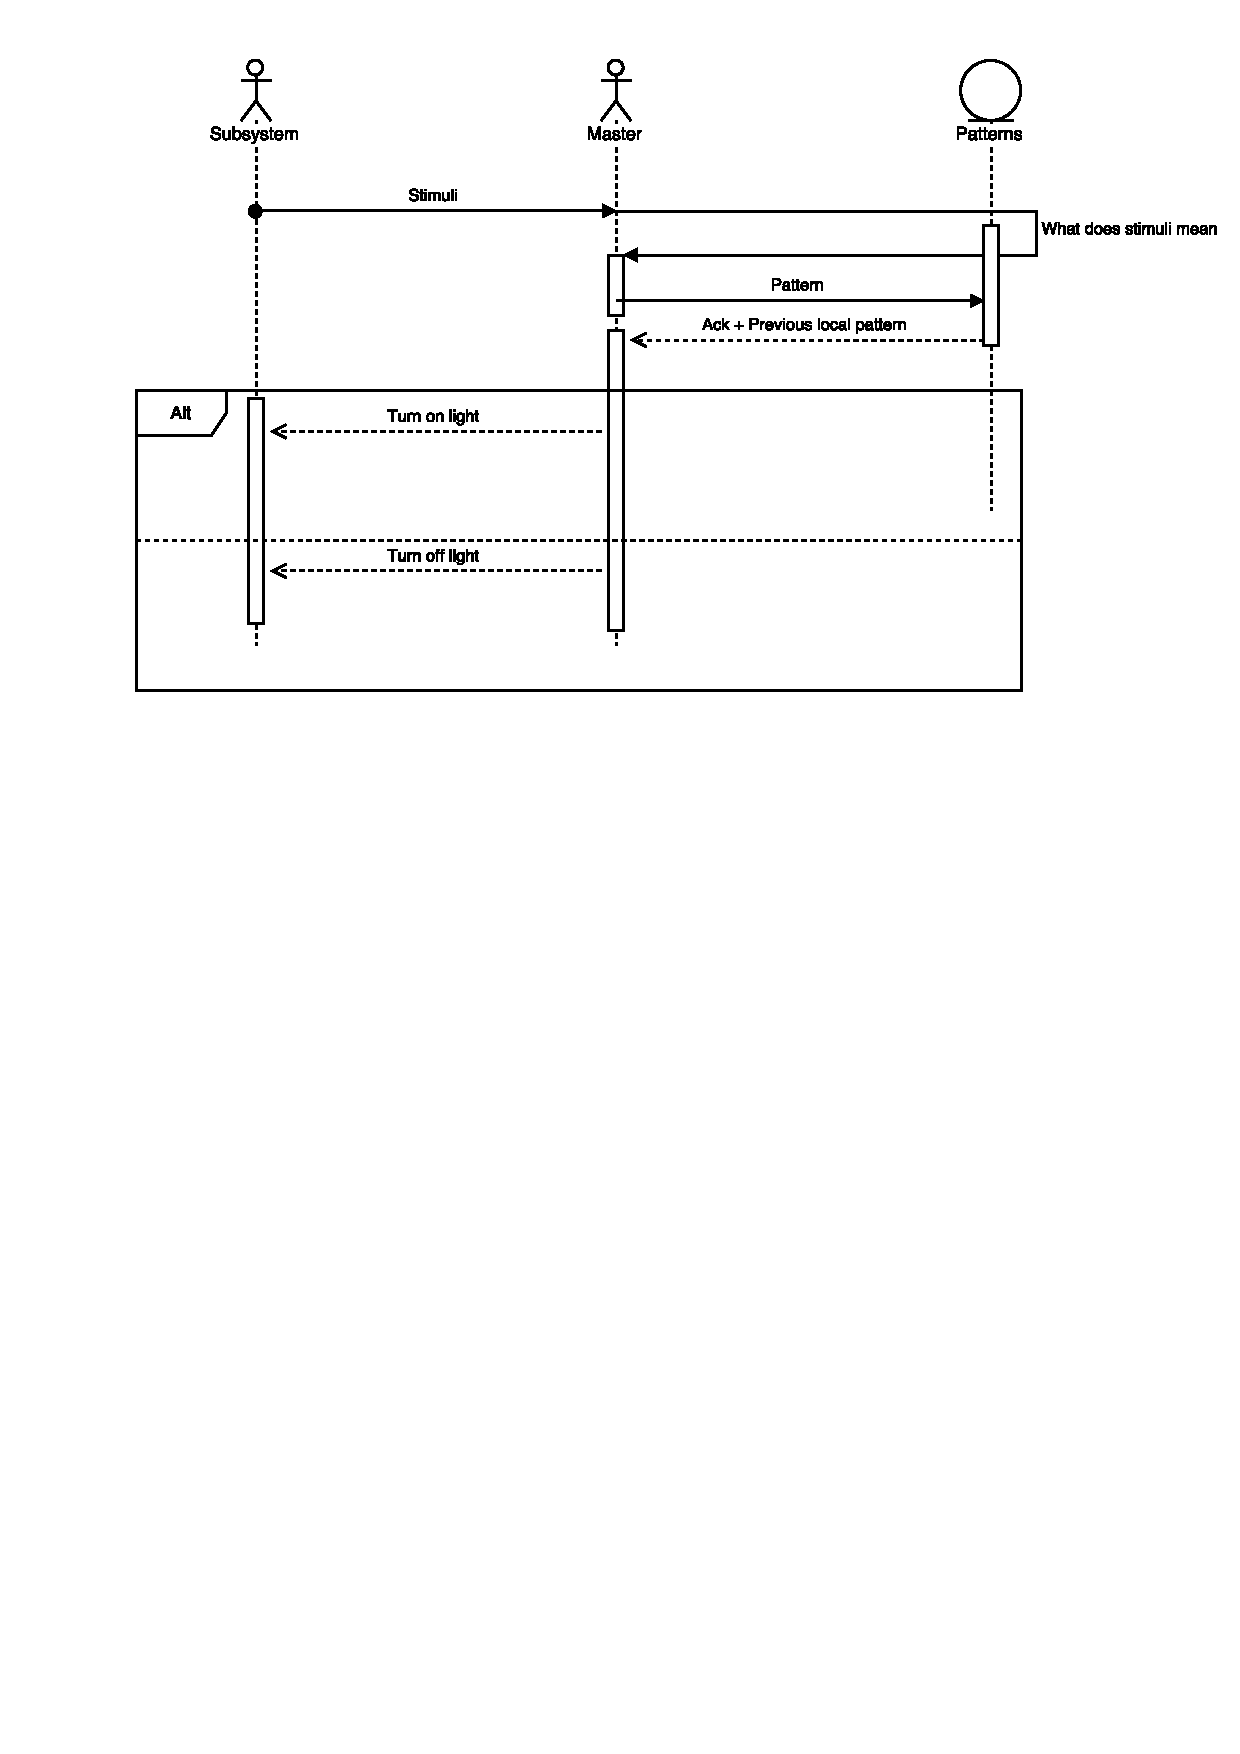
\includegraphics{Behaviour.pdf}
   \end{adjustbox}
   \caption{Behaviour diagram}
\end{figure}
